\documentclass[../main.tex]{subfiles}

Durante este capítulo se explican las diferentes herramientas \emph{software} y \emph{hardware} que han servido de ingredientes en la realización de este trabajo. A la hora de proceder a desgranar los diferentes agentes que entran en acción, se realiza previamente una clasificación entre el lado tierra, el lado aire y la comunicación entre estos que se reflejan en las secciones de este capítulo. \\

\section{Lado Tierra} \label{section:infra-tierra}
El lado tierra se compone por un ordenador donde se ejecuta \emph{UAVCommander}, la aplicación desarrollada. El software se idea como multiplataforma, por lo que el sistema operativo del ordenador puede ser cualquiera de las principales soluciones en el mercado. Sin embargo, la plataforma utilizada durante el desarrollo y las pruebas ha sido Ubuntu, la distribución de Linux basada en Debian. En concreto, la edición utilizada es la última versión con soporte de largo plazo, \textbf{Ubuntu 18.04.3 LTS (\emph{Bionic Beaver})} \cite{ubuntu}. El motivo de esta elección es debido a que Ubuntu suele ser la primera opción en aplicaciones relacionadas con el software libre y la robótica. \\
El lenguaje elegido para el desarrollo de la aplicación ha sido Python \cite{python}. Este lenguaje creado a principios de 1990 por Guido van Rossum en los Países Bajos es un lenguaje de programación interpretado, interactivo y orientado a objetos. Sus principales ventajas, que han motivado su elección para este proyecto, son una sintaxis muy clara y su portabilidad. En concreto, la versión utilizada es \textbf{Python v3.6.9}. \\
Son varias las bibliotecas de Python utilizadas, entre ellas se quiere destacar \textbf{PyQt5} \cite{pyqt}. PyQt5 es un \emph{binding} de la biblioteca gráfica Qt5 \cite{qt} para el lenguaje de programación Python. Qt es un entorno multiplataforma escrito en C++ que permite el desarrollo de interfaces gráficas de usuario de forma sencilla. \\
Otra biblioteca relevante es \textbf{PyMavlink} \cite{pymavlink}, una implementación en Python del protocolo de comunicaciones MAVLink, el cual se explicará más adelante. El uso de esta librería facilita el uso del protocolo de comunicaciones, simplificando el uso de comandos y reduciendo el riesgo de cometer errores. \\
Para el manejo de mapas geo-referenciados se han utilizado diversas librerías. Un mapa geo-referenciado es aquel en el que conocemos o podemos calcular la posición real que representa cada píxel del mismo. Por un lado, se ha utilizado servicios de mapa web (WMS, \emph{Web Map Services}) para obtener las imágenes como \emph{Google Maps Platform} \cite{google-map} u \emph{Open Map Tiles} \cite{open-map} a través de librerías como \emph{urllib} para el manejo de URLs \cite{urlib} o \emph{PIL} (\emph{Python Image Library}) y \emph{Pillow}, para el manejo de imágenes \cite{pil}. \\
Por otro lado, para la lectura de imágenes locales geo-referenciadas procedentes del Instituto Geográfico Nacional (IGN) \cite{ign} a través del Plan Nacional de Ortofotografía Aérea (PNOA) \cite{pnoa} se ha utilizado la librería \textbf{GDAL} \cite{gdal}. GDAL es una biblioteca que permite leer más de 200 formatos de datos geoespaciales ráster y vectoriales, entre los cuales se encuentran formatos como GeoTIFF o ECW, utilizados por la aplicación. \\
Otras librerías utilizadas son \emph{math} \cite{math-python}, \emph{numpy} \cite{numpy}, \emph{threading} \cite{threading-python}, \emph{json} \cite{json-python}, \emph{collections} \cite{collection-python}, \emph{datetime} \cite{datetime-python}, \emph{time} \cite{time-python} o \emph{qfi} \cite{qfi-python}. \\
A la hora de desarrollo se ha utilizado la plataforma GitHub \cite{github} y el entorno de desarrollo PyCharm \cite{pycharm}. GitHub es plataforma de desarrollo colaborativo para alojar proyectos utilizando el sistema de control de versiones Git. % El código fuente del proyecto se encuentra en un repositorio privado debido a que está ligado a un proyecto de desarrollo con una empresa privada. De todas formas, en el siguiente capítulo se presentarán diferentes fragmentos de código mostrando algún aspecto de la implementación. En cambio, la memoria junto con cierta información sobre el trabajo se aloja en un repositorio publico \cite{repo-tfg}. \\
PyCharm es un entorno de desarrollo integrado (IDE, \emph{Integrated Development Environment}), ampliamente utilizado con Python. Entre sus ventajas destacan su depurador, la refactorización, entre otros aspectos.


\section{Lado Aire} \label{section:infra-aire}
El lado aire es el drone. Se distinguen dos posibilidades, el drone puede ser real o simulado. Ambas posibilidades siguen un bucle de control similar. La Figura \ref{fig:loop-control} representa el bucle estándar de control disponible en los autopilotos más comunes. \\

\begin{figure}[h]
    \centering
    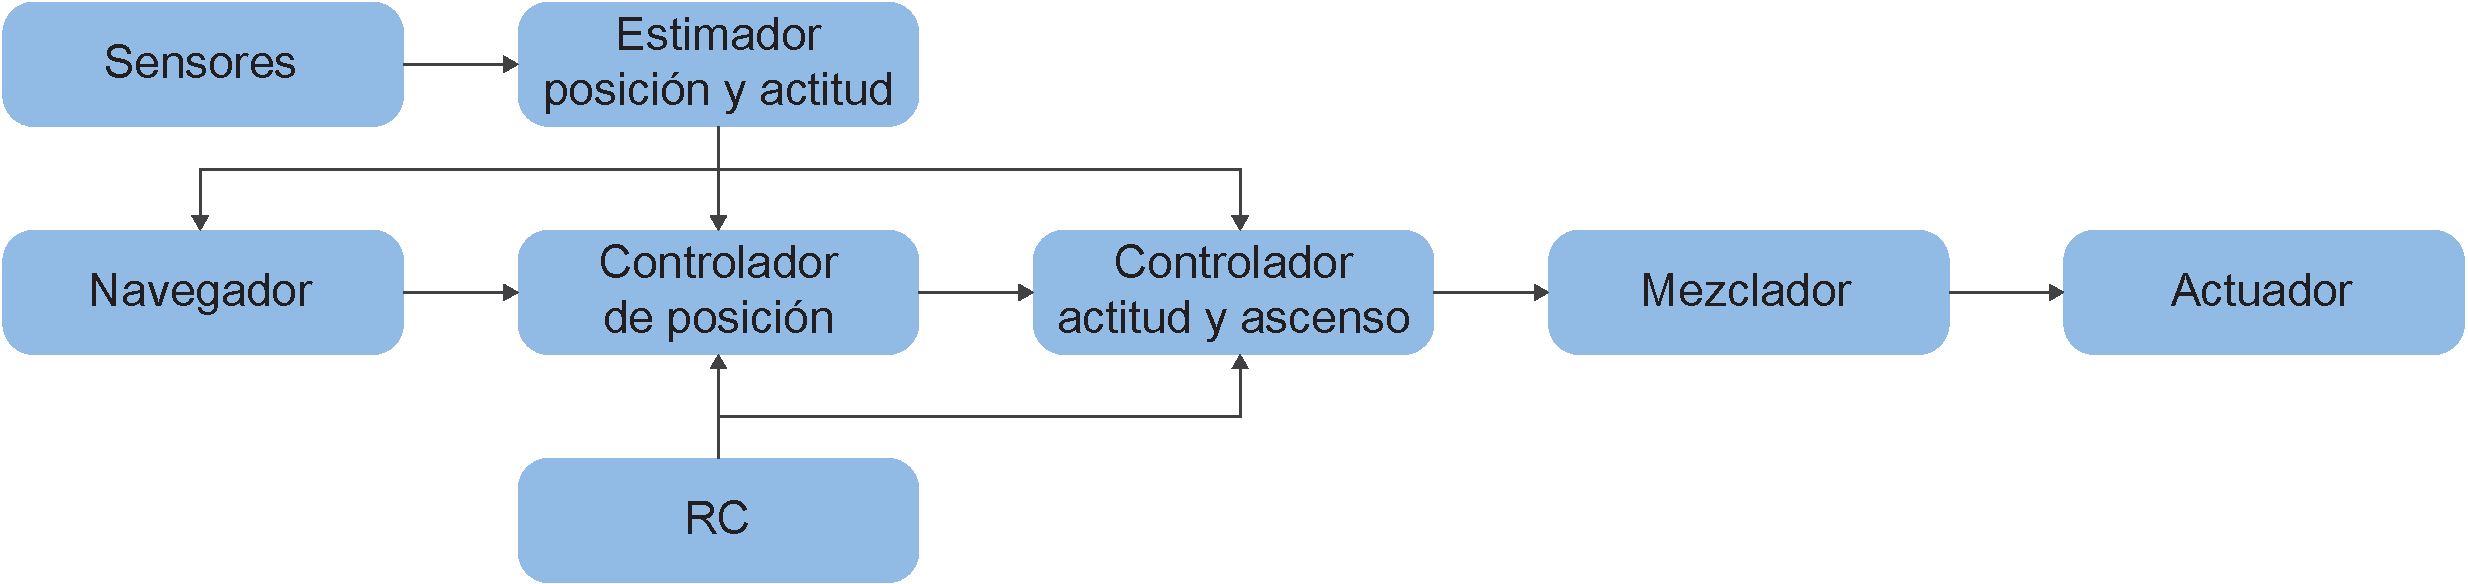
\includegraphics[width=\textwidth]{loop-control.pdf}
    \caption{Bucle de control de un UAV \cite{loop-control}.}
    \label{fig:loop-control}
\end{figure}

El estimador toma una o más entradas de diferentes sensores, las combina y calcula el estado del vehículo. La controladora toma un punto de ajuste y una medición o estado estimado como entradas. Su objetivo es ajustar el valor del estado estimado de modo que coincida con el punto de ajuste. La salida es una corrección para eventualmente alcanzar ese punto de ajuste. Por ejemplo, el controlador de posición toma los puntos de ajuste de posición como entradas, y según la posición estimada calcula la salida que es un punto de ajuste de actitud y empuje que mueve el vehículo hacia la posición deseada. Finalmente, el mezclador toma comandos concretos, como girar a la derecha, y los traduce a comando de motor individuales, al tiempo que garantiza que no se excedan algunos límites. Esta traducción es específica para cada vehículo y depende de varios factores, como la disposición del motor con respecto al centro de gravedad o la inercia rotacional del vehículo. \\

El uso de drone real se ha limitado a las últimas fases de desarrollo de este proyecto, que muy frecuentemente se ha visto sustituido por un drone simulado (ver Fig. \ref{fig:drone-sim}). Sobre el sistema propuesto en la sección anterior (Ubuntu 18.04.3) se ejecuta una simulación en software (\textbf{SITL}, \emph{Software-In-The-Loop}) de una aeronave. El SITL permite enviar y recibir comandos a una controladora sin necesidad de tener el equipo real y evitando la pérdida de la aeronave en caso de error del programa. \\

\begin{figure}[h]
    \centering
    \includegraphics[width=0.8\textwidth]{drone-sim.png}
    \caption{Cuacóptero simulado sobre Gazebo9.}
    \label{fig:drone-sim}
\end{figure}

El firmware utilizado como controladora es \textbf{PX4} \cite{px4}, cuyo esquema de SITL se puede observar en la Figura \ref{fig:sitl-px4}. PX4 es un software de control de vuelo de código abierto para drones y otros vehículos no tripulados. PX4 proporciona un estándar para ofrecer soporte de hardware de drones, lo que permite que un ecosistema construya y mantenga hardware y software de forma escalable. \\

\begin{figure}[H]
    \centering
    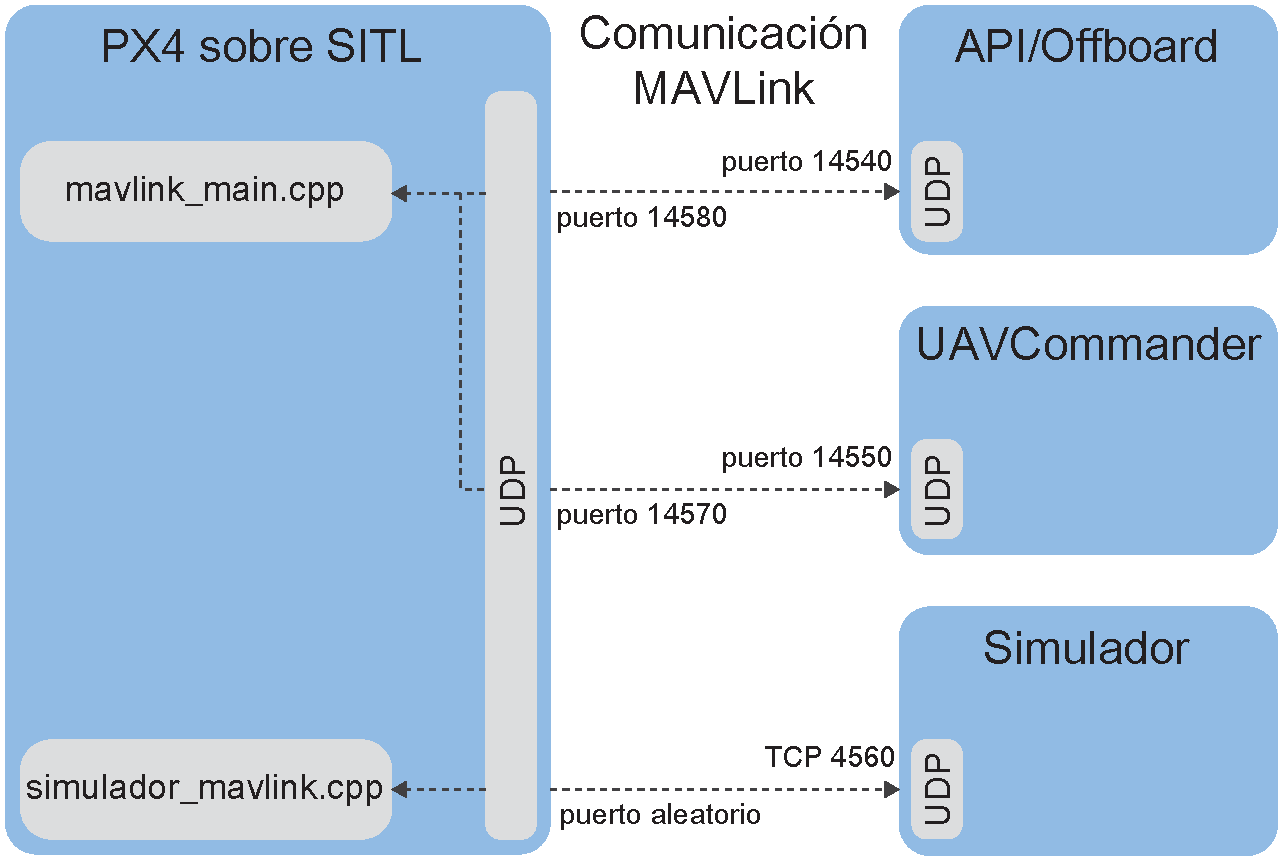
\includegraphics[width=0.7\textwidth]{px4-sitl.pdf}
    \caption{Esquema de PX4 sobre SITL \cite{px4}.}
    \label{fig:sitl-px4}
\end{figure}

Además, la simulación se puede conectar con un simulador para hacer más completa la experiencia y mostrar el vuelo en un entorno de pruebas con elementos del mundo real. Entre los distintos simuladores se ha elegido Gazebo \cite{gazebo}. Este simulador de código abierto es por excelencia el más utilizado en aplicaciones de robótica y visión artificial. Debido a su gestión abierta permite la integración de múltiples vehículos, mundos, sensores, físicas, etc. La versión utilizada durante el proyecto es \textbf{Gazebo9}. \\

La aeronave real puede ser de diversa índole, como ya se ha visto en el capítulo anterior. A lo largo de este proyecto se prevé utilizar:

\begin{itemize}
    \item \textbf{3DR Solo Drone:} Cuadricóptero fabricado por 3DR Robotics \cite{3dr} (Fig. \ref{fig:3dr}). Posee una controladora con firmware Pixhawk v1 \cite{pixhawk} con Ardupilot \cite{ardupilot} \emph{flasheado}, una de las soluciones más usada en el mercado. Una de las principales ventajas que decidieron el uso de este drone en las primeras fases de vuelo frente a otros equipos del laboratorio es la existencia de una emisora (o mando de control), el cual permite controlar la aeronave ante cualquier problema que no este previsto en el software.
    %\item \textbf{Geodrone training:} Aeronave de ala fija (Fig. \ref{fig:geodrone-training}). Posee una controladora con firmware Ardupilot \cite{ardupilot}. Al igual que el anterior, posee una emisora que aporta robustez y permite actuar ante cualquier imprevisto.
    %\item \textbf{PX4:} A completar.
\end{itemize}

\begin{figure}[!ht]
    \begin{subfigure}{\textwidth}
        \centering
        \includegraphics[width=0.7\linewidth]{3dr.jpg}
        \caption{3DR Solo Drone.}
        \label{fig:3dr}
    \end{subfigure}
    %\begin{subfigure}{0.5\textwidth}
    %    \includegraphics[height=6cm, width=0.9\linewidth]{geodrone-training.png}
    %    \caption{Geodrone Training.}
    %    \label{fig:geodrone-training}
    %\end{subfigure}
     
    \caption{Aeronaves utilizadas durante el proyecto.}
    \label{fig:drone-real}
\end{figure}

\section{Protocolo de comunicaciones} \label{section:infra-protoc}
Tal como se ha adelantado, el protocolo de comunicaciones utilizado es MAVLink \cite{mavlink}. MAVLink son las siglas de \emph{Micro Air Vehicle Link}, un protocolo de comunicaciones muy ligero para el intercambio de mensajes con un drone y sus componentes a bordo. La versión utilizada es \textbf{MAVLink v2}. \\
Los extremos de la comunicación se han explicado en las secciones anteriores, siendo este protocolo el puente de comunicación entre el lado tierra y el lado aire. Es considerado como el protocolo estándar de comunicaciones en robótica aérea y las principales soluciones comerciales lo utilizan. Existen diferentes tipos de mensajes, comandos (de navegación, de \emph{perform}, etc.), enumerados y microservicios. \\
Los mensajes son el objeto más pequeño de intercambio de información del protocolo. Son muchos los mensajes existentes y de diversa utilidad. Los diferentes mensajes de MAVLink se pueden observar en su documentación \cite{mavlink-msg}. Un ejemplo de un mensaje MAVLink se puede observar en el Código \ref{listing:msg-exp}.

\begin{listing}[h]
\begin{minted} [frame=lines, framesep=2mm, baselinestretch=1.2, bgcolor=LightGray, fontsize=\footnotesize, linenos]{xml}

<message id="54" name="SAFETY_SET_ALLOWED_AREA">
  <description>Set a safety zone (volume), which is defined by two corners of a cube. 
                This message can be used to tell the MAV which setpoints/waypoints 
                to accept and which to reject. Safety areas are often enforced 
                by national or competition regulations.</description>
  <field type="uint8_t" name="target_system">System ID</field>
  <field type="uint8_t" name="target_component">Component ID</field>
  <field type="uint8_t" name="frame" enum="MAV_FRAME">Coordinate frame. Can be either
                                global, GPS, right-handed with Z axis up or local, 
                                right handed, Z axis down.</field>
  <field type="float" name="p1x" units="m">x position 1 / Latitude 1</field>
  <field type="float" name="p1y" units="m">y position 1 / Longitude 1</field>
  <field type="float" name="p1z" units="m">z position 1 / Altitude 1</field>
  <field type="float" name="p2x" units="m">x position 2 / Latitude 2</field>
  <field type="float" name="p2y" units="m">y position 2 / Longitude 2</field>
  <field type="float" name="p2z" units="m">z position 2 / Altitude 2</field>
</message>
    
\end{minted}
\caption{Mensaje MAVLink tipo.}
\label{listing:msg-exp}
\end{listing}

Existe un tipo especial de mensajes que encapsulan a los comandos, órdenes a ejecutar por la aeronave. Los comandos pueden ser de tres tipos: de navegación, de acción y de condición. Los comandos utilizados en el protocolo se pueden comprobar también en la documentación de MAVLink \cite{mavlink-msg}. Un ejemplo de comando MAVLink se puede observar en el Código \ref{listing:cmd-exp}.

\begin{listing}[h]
\begin{minted} [frame=lines, framesep=2mm, baselinestretch=1.2, bgcolor=LightGray, fontsize=\footnotesize, linenos]{xml}

<enum name="MAV_CMD">
    <description>Commands to be executed by the MAV. They can be executed on user 
                request, or as part of a mission script. If the action is used in 
                a mission, the parameter mapping to the waypoint/mission message is 
                as follows: Param 1, Param 2, Param 3, Param 4, X: Param 5, Y:Param 6,
                Z:Param 7. This command list is similar what ARINC 424 is for 
                commercial aircraft: A data format how to interpret waypoint/mission
                data.</description>
    <entry value="16" name="MAV_CMD_NAV_WAYPOINT">
        <description>Navigate to waypoint.</description>
        <param index="1">Hold time in decimal seconds. (ignored by fixed wing, time 
                        to stay at waypoint for rotary wing)</param>
        <param index="2">Acceptance radius in meters (if the sphere with this radius
                        is hit, the waypoint counts as reached)</param>
        <param index="3">0 to pass through the WP, if &gt; 0 radius in meters to pass
                        by WP. Positive value for clockwise orbit, negative value for
                        counter-clockwise orbit. Allows trajectory control.</param>
        <param index="4">Desired yaw angle at waypoint (rotary wing). NaN for
                        unchanged.</param>
        <param index="5">Latitude</param>
        <param index="6">Longitude</param>
        <param index="7">Altitude</param>
    </entry>
      ...
</enum>
    
\end{minted}
\caption{Comando MAVLink tipo.}
\label{listing:cmd-exp}
\end{listing}

Los enumerados se usan para definir valores con nombre que se pueden usar como opciones en los mensajes, por ejemplo, para representar errores, estados o modos. Cada enumerado tiene un atributo de nombre obligatorio y puede contener una serie de elementos de entrada (con nombres exclusivos de enumeración) para los valores admitidos. Al igual que los mensajes y los comandos, los enumerados disponibles se pueden comprobar en la documentación de MAVLink \cite{mavlink-msg}. \\
Finalmente, los microservicios representan protocolos de alto nivel que los sistemas MAVLink pueden adoptar para una mejor interacción. Los microservicios se utilizan para intercambiar muchos tipos de datos, incluidos: parámetros, misiones, trayectorias, imágenes y otros archivos. Los datos pueden ser mucho más grandes de lo que cabe en un solo mensaje, por lo que los microservicios definirán cómo se dividen y se vuelven a ensamblar los datos, y cómo garantizar que los datos perdidos se vuelvan a transmitir. Otros microservicios proporcionan reconocimiento de comandos, informes de errores, etc. Los diferentes microservicios se definen en la documentación de MAVLink \cite{mavlink-microserv}.
